\chapter{LLM Pre-Training --- From Raw Text to World Models}
\label{ch:pretraining}

\noindent
On day 47 of a 65-day training run, the loss curve spiked. Not a small blip---the kind of spike that erases three days of progress in thirty seconds. The training cluster---4,096 H100 GPUs rented at \$2 per GPU-hour---was burning \$196,000 per day. The team had 20 minutes to decide: roll back to the checkpoint from 12 hours ago (losing \$98,000 of compute), or hope the spike was transient and the loss would recover on its own.

It didn't recover. They rolled back, diagnosed the cause (a corrupted data shard in the 14th epoch of their code subset that contained a 2GB auto-generated file of the same line repeated 50 million times), fixed the data pipeline, and resumed. Total cost of the incident: roughly \$150,000 and two days of calendar time. Nobody wrote a postmortem. This is just Tuesday in pre-training.

Pre-training is where a language model acquires its fundamental capabilities. It is the most expensive, most computationally demanding, and most consequential phase of the LLM lifecycle. A pre-training run for a frontier model costs tens to hundreds of millions of dollars, consumes megawatts of power for months, and involves coordinating thousands of accelerators in a fault-tolerant distributed system that would make any distributed systems engineer's head spin.

This chapter explains pre-training from a software engineer's perspective. We are not interested in deriving the attention mechanism from first principles---there are excellent textbooks for that. Instead, we focus on the \emph{systems} aspects: how training data is processed at petabyte scale, how the transformer architecture translates to actual compute operations, how distributed training coordinates thousands of GPUs, and what the infrastructure looks like in practice. If you've ever designed a distributed database or managed a Kubernetes cluster at scale, you already have the right mental models. The concepts are the same---partitioning, replication, fault tolerance, observability---only the workload is different.


\section{The Training Data Pipeline}
\label{sec:training-data}

A language model is only as good as its training data. The data pipeline for pre-training a modern LLM is a massive-scale ETL system that processes petabytes of text from diverse sources and produces a clean, deduplicated, carefully balanced training corpus. Understanding this pipeline is essential for software engineers because it reveals both the capabilities and limitations of the resulting model.

\subsection{Data Collection}

The starting point for most pre-training corpora is a web crawl---typically Common Crawl, which archives billions of web pages. But raw web data is extraordinarily noisy: it includes spam, SEO-optimized garbage, navigation menus, cookie consent banners, duplicated content, and text in hundreds of languages with varying quality.

A typical data collection pipeline processes multiple sources:

\begin{itemize}[leftmargin=*]
    \item \textbf{Web crawls}: Common Crawl, internal crawls (Google, etc.)
    \item \textbf{Books}: Digitized books, often from the Internet Archive or publisher partnerships
    \item \textbf{Code}: GitHub repositories, often filtered by license and quality
    \item \textbf{Scientific literature}: ArXiv, PubMed, Semantic Scholar
    \item \textbf{Wikipedia}: High-quality encyclopedic content in multiple languages
    \item \textbf{Curated datasets}: StackOverflow, Reddit, specialized forums
    \item \textbf{Synthetic data}: Increasingly, data generated by existing models
\end{itemize}

The LLaMA training corpus~\cite{touvron2023llama} provides a useful reference for the proportions: approximately 67\% web data, 15\% code, 4.5\% Wikipedia, 4.5\% books, 2.5\% ArXiv, and 6.5\% StackExchange and other curated sources.

\subsection{Data Cleaning and Filtering}

Raw data must be aggressively cleaned. A production data pipeline typically applies the following stages:

\begin{enumerate}[leftmargin=*]
    \item \textbf{Language identification}: Classify documents by language using fastText or similar classifiers. Remove documents in languages not targeted for the model.
    \item \textbf{Quality filtering}: Remove low-quality documents using a combination of heuristic rules and trained quality classifiers:
    \begin{itemize}
        \item Perplexity filtering: Remove documents with very high perplexity (likely garbled text)
        \item Length filtering: Remove very short documents (likely navigation fragments) and very long ones (likely data dumps)
        \item Special character ratio: Remove documents with excessive URLs, HTML tags, or non-alphabetic characters
        \item Repetition filtering: Remove documents with excessive n-gram repetition (``buy now buy now buy now'')
    \end{itemize}
    \item \textbf{Content filtering}: Remove toxic, biased, or personally identifiable content using classifiers and keyword lists
    \item \textbf{Deduplication}: Perhaps the most critical step---duplicated data causes the model to memorize rather than generalize
\end{enumerate}

\begin{lstlisting}[language=Python, caption={Simplified quality filtering pipeline}]
from dataclasses import dataclass
from typing import Iterator

@dataclass
class Document:
    text: str
    source: str
    language: str
    url: str | None = None

def quality_filter(docs: Iterator[Document]) -> Iterator[Document]:
    """Multi-stage quality filtering pipeline."""
    for doc in docs:
        # Stage 1: Basic heuristics
        if len(doc.text) < 100 or len(doc.text) > 500_000:
            continue
        
        words = doc.text.split()
        if len(words) < 20:
            continue
        
        # Stage 2: Special character ratio
        alpha_ratio = sum(c.isalpha() for c in doc.text) / len(doc.text)
        if alpha_ratio < 0.6:
            continue
        
        # Stage 3: Repetition check (unigram entropy)
        unique_words = set(w.lower() for w in words)
        uniqueness_ratio = len(unique_words) / len(words)
        if uniqueness_ratio < 0.1:  # Extremely repetitive
            continue
        
        # Stage 4: Perplexity check (via small reference model)
        perplexity = compute_perplexity(doc.text)
        if perplexity > 10_000:  # Likely garbled
            continue
        
        yield doc
\end{lstlisting}

\subsection{Deduplication}

Deduplication is critical because duplicated training data has several harmful effects:

\begin{itemize}[leftmargin=*]
    \item \textbf{Memorization}: The model memorizes exact sequences rather than learning general patterns, increasing the risk of verbatim output of copyrighted or private content
    \item \textbf{Training instability}: Duplicated data creates ``hot spots'' that distort gradient updates
    \item \textbf{Wasted compute}: Training on duplicated data is literally burning money on content the model has already seen
\end{itemize}

Three main deduplication strategies are used in practice:

\textbf{Exact deduplication} removes documents that are byte-for-byte identical. This is trivially implemented with hash maps but catches only the most obvious duplicates.

\textbf{Near-deduplication} catches documents that differ only slightly (e.g., the same article with different ads or timestamps). The standard approach uses MinHash with Locality-Sensitive Hashing (LSH):

\begin{lstlisting}[language=Python, caption={MinHash-based near-deduplication (simplified)}]
from datasketch import MinHash, MinHashLSH

def create_minhash(text: str, num_perm: int = 128) -> MinHash:
    """Create MinHash signature for a document."""
    m = MinHash(num_perm=num_perm)
    # Use word-level 5-grams as features
    words = text.lower().split()
    for i in range(len(words) - 4):
        ngram = " ".join(words[i:i+5])
        m.update(ngram.encode('utf-8'))
    return m

def deduplicate(documents: list[Document], 
                threshold: float = 0.8) -> list[Document]:
    """Remove near-duplicate documents using MinHash LSH."""
    lsh = MinHashLSH(threshold=threshold, num_perm=128)
    unique_docs = []
    
    for i, doc in enumerate(documents):
        mh = create_minhash(doc.text)
        # Check if similar document already exists
        result = lsh.query(mh)
        if not result:
            lsh.insert(f"doc_{i}", mh)
            unique_docs.append(doc)
    
    return unique_docs
\end{lstlisting}

\textbf{Substring deduplication} removes repeated sequences \emph{within} and across documents using suffix arrays. This catches boilerplate content like legal disclaimers and navigation text that appear across many web pages.

\begin{keytakeaway}
The data pipeline for pre-training is a petabyte-scale ETL system. It requires the same engineering rigor as any production data system: monitoring, testing, versioning, and quality assurance. Engineers who understand data pipelines have a significant advantage in understanding LLM capabilities and limitations.
\end{keytakeaway}

\section{Tokenization}
\label{sec:tokenization}

Before text can be fed into a neural network, it must be converted into a sequence of integers---a process called \term{tokenization}. Tokenization is one of the most underappreciated design decisions in the LLM stack, and it has far-reaching consequences for model performance, cost, and behavior.

\subsection{Why Not Just Use Characters or Words?}

Character-level tokenization (one integer per character) creates extremely long sequences. The sentence ``Software engineering is evolving'' becomes 35 tokens. Since transformer attention is quadratic in sequence length ($O(n^2)$), this is prohibitively expensive.

Word-level tokenization creates a fixed vocabulary of known words, but struggles with:
\begin{itemize}[leftmargin=*]
    \item \textbf{Out-of-vocabulary words}: New words, misspellings, and technical terms get mapped to a generic \code{<UNK>} token
    \item \textbf{Morphological variants}: ``running,'' ``runs,'' ``ran'' are all separate vocabulary entries
    \item \textbf{Multilingual text}: Chinese, Japanese, and other languages don't have clear word boundaries
    \item \textbf{Code}: Programming languages have virtually infinite ``words'' (variable names, function names)
\end{itemize}

\subsection{Byte Pair Encoding (BPE)}

The standard solution is \term{Byte Pair Encoding} (BPE)~\cite{sennrich2016bpe}, a subword tokenization algorithm. BPE works by iteratively merging the most frequent adjacent pairs of tokens, starting from individual bytes:

\begin{enumerate}[leftmargin=*]
    \item Start with a vocabulary of 256 byte-level tokens
    \item Scan the training corpus and find the most frequent adjacent pair (e.g., ``t'' + ``h'' $\rightarrow$ ``th'')
    \item Add the merged token to the vocabulary
    \item Replace all occurrences of the pair in the corpus
    \item Repeat until the desired vocabulary size is reached (typically 32K--128K tokens)
\end{enumerate}

\begin{lstlisting}[language=Python, caption={Simplified BPE training algorithm}]
from collections import Counter

def train_bpe(text: str, num_merges: int) -> dict[tuple, str]:
    """Train a BPE tokenizer from scratch."""
    # Initialize: split text into characters
    tokens = list(text.encode('utf-8'))
    merges = {}
    
    for i in range(num_merges):
        # Count all adjacent pairs
        pairs = Counter()
        for j in range(len(tokens) - 1):
            pairs[(tokens[j], tokens[j + 1])] += 1
        
        if not pairs:
            break
        
        # Find most frequent pair
        best_pair = pairs.most_common(1)[0][0]
        new_token = 256 + i  # New token ID
        merges[best_pair] = new_token
        
        # Replace all occurrences of the pair
        new_tokens = []
        j = 0
        while j < len(tokens):
            if (j < len(tokens) - 1 and 
                (tokens[j], tokens[j + 1]) == best_pair):
                new_tokens.append(new_token)
                j += 2
            else:
                new_tokens.append(tokens[j])
                j += 1
        tokens = new_tokens
    
    return merges
\end{lstlisting}

The key insight is that BPE creates a vocabulary that reflects the frequency distribution of the training data. Common words (``the,'' ``and,'' ``is'') become single tokens. Rare words are broken into subword pieces that can be recombined. This gives the model a flexible, efficient representation that works across languages and domains.

\subsection{Tokenizer Design Trade-offs}

\begin{table}[htbp]
\centering
\caption{Tokenizer vocabulary sizes across major LLMs}
\label{tab:tokenizer-sizes}
\begin{tabularx}{\textwidth}{lrX}
\toprule
\textbf{Model} & \textbf{Vocab Size} & \textbf{Notable Design Choices} \\
\midrule
GPT-2       & 50,257  & BPE on English-heavy data; poor multilingual support \\
GPT-4       & 100,256 & Improved multilingual coverage; better code tokenization \\
LLaMA       & 32,000  & SentencePiece BPE; byte-fallback for unknown characters \\
LLaMA 3     & 128,256 & Larger vocab for better multilingual \& code efficiency \\
Gemini      & 256,000 & Very large vocab; SentencePiece; excellent multilingual \\
Mistral     & 32,768  & SentencePiece BPE; compact vocabulary \\
\bottomrule
\end{tabularx}
\end{table}

\begin{cautionbox}
Tokenization directly affects cost and latency. The same text can require 30\% more tokens with GPT-2's tokenizer than with GPT-4's, simply because the vocabulary was trained on different data. For multilingual applications, this difference can be 2--3x. Always profile token counts for your specific use case.
\end{cautionbox}

\section{The Transformer Architecture: A Systems Perspective}
\label{sec:transformer}

The transformer~\cite{vaswani2017attention} is the neural network architecture that underlies all modern LLMs. While the mathematical details are well-covered elsewhere, software engineers benefit from understanding the transformer as a \emph{system}---a pipeline of well-defined operations with specific computational costs, memory requirements, and parallelization properties.

\subsection{The Forward Pass as a Data Pipeline}

A transformer processes an input sequence through a series of layers, each consisting of two main operations: \emph{self-attention} and a \emph{feed-forward network}. From a systems perspective, this is a pipeline:

\begin{figure}[htbp]
\centering
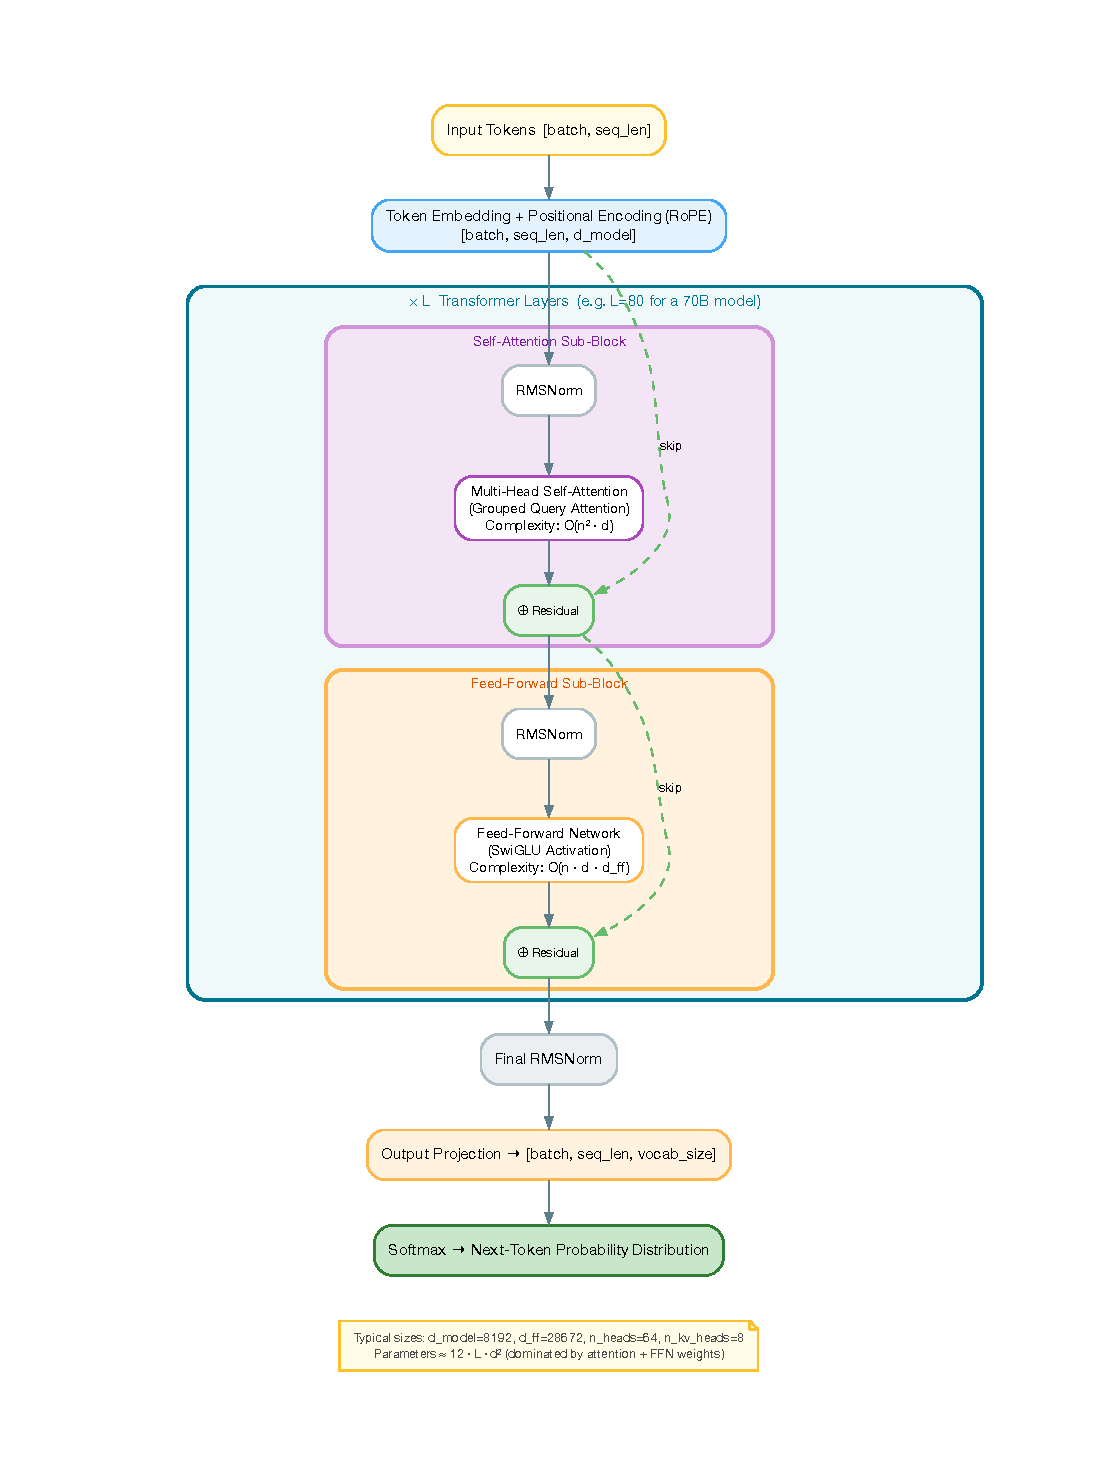
\includegraphics[width=\textwidth]{diagrams/compiled/ch02/transformer-arch.pdf}
\caption{The transformer architecture viewed as a data processing pipeline}
\label{fig:transformer-arch}
\end{figure}

\begin{enumerate}[leftmargin=*]
    \item \textbf{Token embedding}: Each token ID is mapped to a dense vector (lookup table). $O(V \times d)$ parameters, where $V$ is vocabulary size and $d$ is the model dimension.
    \item \textbf{Positional encoding}: Position information is added to the embeddings, since attention is inherently position-agnostic. Modern models use Rotary Position Embeddings (RoPE) rather than the sinusoidal encodings of the original transformer.
    \item \textbf{Self-attention} (repeated $L$ times): The core operation. Each token attends to all other tokens in the sequence, computing weighted sums. $O(n^2 \cdot d)$ computation, $O(n^2)$ memory for the attention matrix.
    \item \textbf{Feed-forward network} (repeated $L$ times): Two linear transformations with a non-linearity. $O(n \cdot d \cdot d_{ff})$ computation, where $d_{ff}$ is typically $4d$.
    \item \textbf{Output projection}: Linear transformation to vocabulary size, followed by softmax to produce next-token probabilities.
\end{enumerate}

\subsection{Attention as a Database Query}

One of the most useful mental models for software engineers is to think of self-attention as a \emph{database query}. In a traditional database:

\begin{itemize}[leftmargin=*]
    \item You have a \textbf{query} (Q): ``Find all products where category = electronics''
    \item The database has \textbf{keys} (K): The indexed columns
    \item When a key matches the query, you retrieve the corresponding \textbf{value} (V)
\end{itemize}

Self-attention works the same way, but with soft (differentiable) matching:

\begin{lstlisting}[language=Python, caption={Self-attention as a soft database lookup}]
import torch
import torch.nn.functional as F

def self_attention(x: torch.Tensor, 
                   W_q: torch.Tensor, 
                   W_k: torch.Tensor, 
                   W_v: torch.Tensor) -> torch.Tensor:
    """
    Self-attention: each token "queries" all other tokens.
    
    x: [batch, seq_len, d_model] - input embeddings
    W_q, W_k, W_v: [d_model, d_k] - projection matrices
    Returns: [batch, seq_len, d_k] - attended representations
    """
    Q = x @ W_q  # What am I looking for?
    K = x @ W_k  # What do I have to offer?
    V = x @ W_v  # What's my actual content?
    
    d_k = Q.shape[-1]
    
    # Soft matching: how well does each query match each key?
    attention_scores = (Q @ K.transpose(-2, -1)) / (d_k ** 0.5)
    
    # For autoregressive models: can only attend to past tokens
    mask = torch.triu(torch.ones_like(attention_scores), diagonal=1)
    attention_scores = attention_scores.masked_fill(mask == 1, float('-inf'))
    
    # Normalize to probabilities
    attention_weights = F.softmax(attention_scores, dim=-1)
    
    # Retrieve weighted values
    return attention_weights @ V
\end{lstlisting}

The key difference from a database is that attention does \emph{soft} matching---every query partially matches every key, and the result is a weighted average of all values. This is what makes transformers so powerful: they can learn complex, context-dependent relationships between tokens.

\subsection{Multi-Head Attention: Parallel Queries}

In practice, the model runs multiple attention ``heads'' in parallel, each with its own Q, K, V projections. This is analogous to running multiple database queries simultaneously, each looking for different types of relationships. One head might learn to attend to syntactic relationships (subject $\rightarrow$ verb), another to semantic relationships (pronoun $\rightarrow$ referent), and another to positional patterns.

\subsection{Scaling Laws: Bigger is (Usually) Better}

One of the most important empirical findings in LLM development is that model performance scales predictably with three factors~\cite{kaplan2020scaling}:

\begin{enumerate}[leftmargin=*]
    \item \textbf{Parameters ($N$)}: The number of learnable weights in the model
    \item \textbf{Data ($D$)}: The number of tokens in the training corpus
    \item \textbf{Compute ($C$)}: The total floating-point operations used for training
\end{enumerate}

The relationship follows a power law: $L \propto N^{-\alpha} + D^{-\beta} + C^{-\gamma}$, where $L$ is the loss and $\alpha$, $\beta$, $\gamma$ are empirically determined exponents.

The Chinchilla scaling laws~\cite{hoffmann2022chinchilla} refined this finding by showing that for a given compute budget, the optimal strategy is to scale both model size and data proportionally. Specifically, for a compute-optimal model, the number of training tokens should be approximately 20x the number of parameters. This means a 7B parameter model should be trained on approximately 140B tokens, and a 70B model on approximately 1.4T tokens.

\begin{table}[htbp]
\centering
\caption{Approximate specifications of major pre-trained models}
\label{tab:model-specs}
\begin{tabularx}{\textwidth}{lrrrrX}
\toprule
\textbf{Model} & \textbf{Params} & \textbf{Tokens} & \textbf{GPUs} & \textbf{Est. Cost} & \textbf{Training Time} \\
\midrule
GPT-3        & 175B   & 300B    & $\sim$1,024 V100 & $\sim$\$5M     & $\sim$34 days \\
LLaMA 2 70B  & 70B    & 2T      & 2,048 A100  & $\sim$\$3M     & $\sim$25 days \\
LLaMA 3 405B & 405B   & 15T+    & 16,384 H100 & $\sim$\$100M+  & $\sim$54 days \\
Gemini Ultra  & $\sim$1T+ & N/A  & TPU v5p pods & $\sim$\$200M+  & Months \\
GPT-4        & $\sim$1.7T (MoE) & $\sim$13T & $\sim$25,000 A100 & $\sim$\$100M+ & $\sim$100 days \\
\bottomrule
\end{tabularx}
\end{table}

\begin{cautionbox}
The cost estimates in Table~\ref{tab:model-specs} are approximate and based on publicly available information, leaked details, and informed estimates. Exact figures are closely guarded trade secrets.
\end{cautionbox}

\section{Pre-Training Infrastructure at Scale}
\label{sec:training-infra}

Training a frontier LLM is one of the most demanding distributed systems engineering challenges in existence. The infrastructure must coordinate thousands of accelerators, handle petabytes of data, maintain numerical stability across weeks of continuous computation, and recover gracefully from hardware failures that occur daily at this scale.

\subsection{Distributed Training Strategies}

A single GPU (even an H100 with 80GB of memory) cannot hold a large language model. A 70B parameter model in 16-bit precision requires approximately 140GB just for the model weights---before accounting for optimizer states, gradients, and activations. Training such a model requires distributing the work across many GPUs using a combination of parallelism strategies.

\begin{figure}[htbp]
\centering
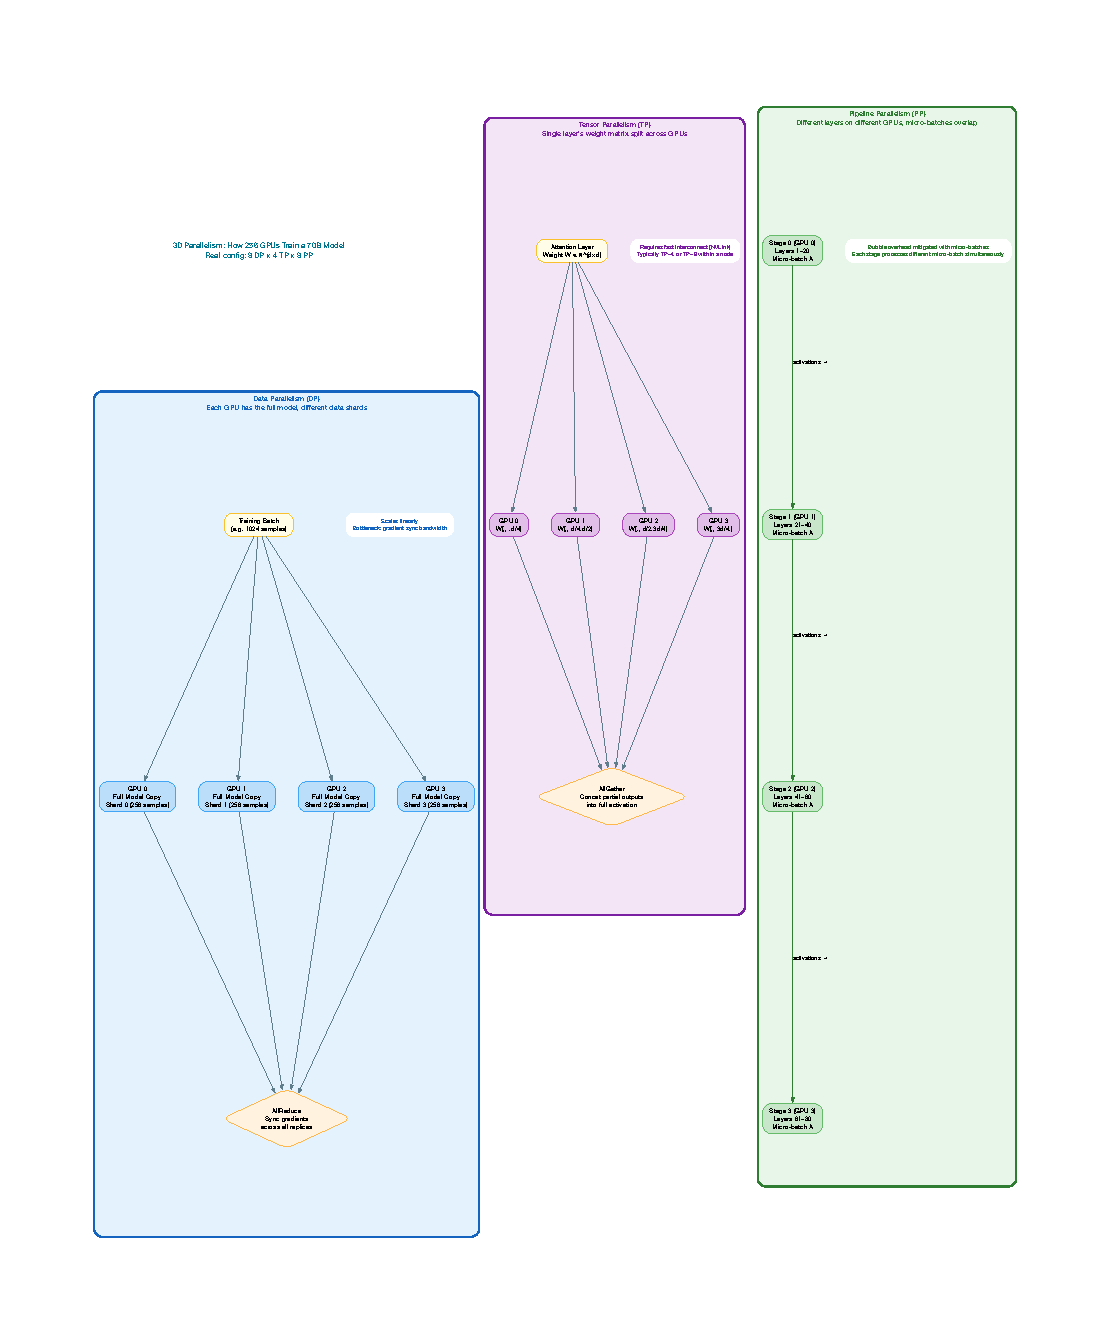
\includegraphics[width=\textwidth]{diagrams/compiled/ch02/distributed-training.pdf}
\caption{The three axes of parallelism in distributed training}
\label{fig:distributed-training}
\end{figure}

\subsubsection{Data Parallelism}

The simplest strategy: replicate the entire model on every GPU, and split the training data across GPUs. Each GPU processes a different mini-batch, computes gradients, and then all GPUs synchronize their gradients via an AllReduce operation.

\begin{lstlisting}[language=Python, caption={Conceptual data parallelism}]
# Pseudocode: Data parallelism
for epoch in range(num_epochs):
    for batch in data_loader:
        # Each GPU gets a different slice of the batch
        local_batch = batch[rank::world_size]
        
        # Forward + backward on local data
        loss = model(local_batch)
        loss.backward()
        
        # Synchronize gradients across all GPUs
        all_reduce(model.gradients)  # O(params * world_size)
        
        optimizer.step()
\end{lstlisting}

Data parallelism scales well but has two limitations: (1) the model must fit on a single GPU, and (2) the AllReduce communication overhead grows with the number of GPUs and model size. Modern systems use \textbf{ZeRO} (Zero Redundancy Optimizer) to shard optimizer states and gradients across GPUs, significantly reducing per-GPU memory requirements.

\subsubsection{Tensor Parallelism}

When a single layer is too large for one GPU, \term{tensor parallelism} splits individual matrix multiplications across GPUs. For example, a linear layer $Y = XW$ with weight matrix $W \in \mathbb{R}^{d \times d}$ can be split column-wise:

$$W = [W_1 | W_2], \quad Y = [XW_1 | XW_2]$$

Each GPU computes half the output, and the results are concatenated. This requires high-bandwidth communication between GPUs within a node, making it best suited for GPUs connected via NVLink ($\sim$900 GB/s on H100 systems).

\subsubsection{Pipeline Parallelism}

\term{Pipeline parallelism} assigns different layers of the model to different GPUs. GPU 0 processes layers 1--10, GPU 1 processes layers 11--20, and so on. This creates a pipeline similar to a CPU instruction pipeline, with micro-batches flowing through the stages.

The main challenge is \emph{pipeline bubbles}: when the pipeline is filling or draining, some GPUs are idle. Modern systems minimize bubbles using techniques like 1F1B (one forward, one backward) scheduling and interleaved stages.

\subsection{Hardware: The GPU Cluster}

A modern training cluster is built from tightly networked nodes, each containing multiple high-end GPUs:

\begin{itemize}[leftmargin=*]
    \item \textbf{GPU}: NVIDIA H100 (80GB HBM3, 990 TFLOPS FP16) or Google TPU v5p
    \item \textbf{Intra-node interconnect}: NVLink/NVSwitch ($\sim$900 GB/s per GPU)
    \item \textbf{Inter-node interconnect}: InfiniBand HDR/NDR (400--800 Gbps per node)
    \item \textbf{Node configuration}: Typically 8 GPUs per node (DGX H100)
    \item \textbf{Cluster scale}: 1,000--25,000+ GPUs for frontier model training
\end{itemize}

The networking topology is critical. Tensor parallelism requires the highest bandwidth (NVLink within a node). Data parallelism AllReduce can tolerate lower bandwidth (InfiniBand across nodes). Pipeline parallelism falls in between.

\subsection{Checkpointing and Fault Tolerance}

At the scale of thousands of GPUs running for weeks, hardware failures are not exceptions---they are the norm. A cluster of 10,000 GPUs might experience multiple GPU failures per day, along with network issues, power fluctuations, and software bugs.

\begin{lstlisting}[language=Python, caption={Checkpoint management for large-scale training}]
import os
import torch
from datetime import datetime, timedelta

class CheckpointManager:
    """Manages periodic checkpointing for fault tolerance."""
    
    def __init__(self, 
                 save_dir: str,
                 save_interval_minutes: int = 30,
                 keep_last_n: int = 5):
        self.save_dir = save_dir
        self.save_interval = timedelta(minutes=save_interval_minutes)
        self.keep_last_n = keep_last_n
        self.last_save_time = datetime.now()
    
    def should_save(self) -> bool:
        return datetime.now() - self.last_save_time > self.save_interval
    
    def save(self, model, optimizer, step: int, loss: float):
        """Save distributed checkpoint (each rank saves its shard)."""
        rank = torch.distributed.get_rank()
        ckpt_dir = os.path.join(
            self.save_dir, f"step_{step:08d}"
        )
        os.makedirs(ckpt_dir, exist_ok=True)
        
        state = {
            'step': step,
            'loss': loss,
            'model_shard': model.state_dict(),
            'optimizer_shard': optimizer.state_dict(),
            'timestamp': datetime.now().isoformat(),
        }
        
        path = os.path.join(ckpt_dir, f"rank_{rank:04d}.pt")
        torch.save(state, path)
        
        # Barrier: wait for all ranks to finish saving
        torch.distributed.barrier()
        
        if rank == 0:
            self._cleanup_old_checkpoints()
        
        self.last_save_time = datetime.now()
    
    def _cleanup_old_checkpoints(self):
        """Keep only the N most recent checkpoints."""
        ckpt_dirs = sorted(
            [d for d in os.listdir(self.save_dir) 
             if d.startswith("step_")]
        )
        for old_dir in ckpt_dirs[:-self.keep_last_n]:
            shutil.rmtree(
                os.path.join(self.save_dir, old_dir)
            )
\end{lstlisting}

\begin{keytakeaway}
Pre-training infrastructure is fundamentally a distributed systems problem. The same principles that apply to distributed databases---partitioning, replication, consensus, fault tolerance---apply to distributed training. Engineers with distributed systems experience are well-equipped to understand and contribute to training infrastructure.
\end{keytakeaway}

\section{Training Dynamics and Stability}
\label{sec:training-dynamics}

Training a large language model is not simply a matter of running gradient descent for a fixed number of steps. The training process itself requires careful monitoring and intervention---it is closer to operating a complex system than running an algorithm.

\subsection{Loss Curves and Monitoring}

The primary signal during training is the \emph{training loss}---the cross-entropy loss between the model's predictions and the actual next tokens. A healthy training run shows a smooth, monotonically decreasing loss curve. But in practice, training runs frequently encounter:

\begin{itemize}[leftmargin=*]
    \item \textbf{Loss spikes}: Sudden jumps in loss, often caused by data quality issues (corrupted batches), learning rate problems, or numerical instability. Teams typically roll back to the last checkpoint before the spike and resume with a lower learning rate.
    \item \textbf{Slow divergence}: The loss starts increasing gradually, often too slowly to notice in real-time dashboards. This can be caused by learning rate schedules that don't decay fast enough or by data distribution shifts in the training corpus.
    \item \textbf{NaN gradients}: Floating-point overflow in gradient computation, typically in mixed-precision training. Modern frameworks detect and skip NaN batches automatically.
\end{itemize}

\subsection{Learning Rate Schedule}

The learning rate schedule is one of the most critical hyperparameters. Most large-scale training runs use a warmup-cosine schedule:

\begin{enumerate}[leftmargin=*]
    \item \textbf{Warmup} (first 0.1--1\% of training): Linearly increase the learning rate from near-zero to the peak value. This prevents early instability when the model's parameters are randomly initialized.
    \item \textbf{Cosine decay}: Smoothly decrease the learning rate following a cosine curve to near-zero by the end of training.
\end{enumerate}

Peak learning rates are typically in the range of 1e-4 to 3e-4 for large models. Higher learning rates train faster but risk instability; lower learning rates are more stable but waste compute.

\subsection{Mixed-Precision Training}

All modern large-scale training uses mixed-precision arithmetic to reduce memory and increase throughput:

\begin{itemize}[leftmargin=*]
    \item \textbf{Forward pass}: FP16 or BF16 (bfloat16). BF16 is preferred because it has the same exponent range as FP32, reducing overflow risk.
    \item \textbf{Weight master copy}: FP32. Used for accumulating small gradient updates that would be lost in lower precision.
    \item \textbf{Loss scaling}: The loss is multiplied by a large factor before backpropagation to prevent gradient underflow in FP16, then the gradients are scaled back down before the optimizer step.
\end{itemize}

\section{Inference: The KV-Cache and Why It Matters}
\label{sec:kv-cache}

Understanding the KV-cache is essential for engineers who deploy and operate LLM-based systems, because it determines the memory requirements and latency characteristics of inference.

During autoregressive generation, the model produces one token at a time. For each new token, the self-attention mechanism needs to attend to \emph{all} previous tokens. Naively, this means recomputing the key and value projections for every past token at every step---an $O(n^2)$ operation that makes generation painfully slow.

The KV-cache eliminates this redundancy by caching the key and value vectors from previous steps. Once a token has been processed, its K and V vectors are stored and reused for all subsequent tokens.

\begin{figure}[htbp]
\centering
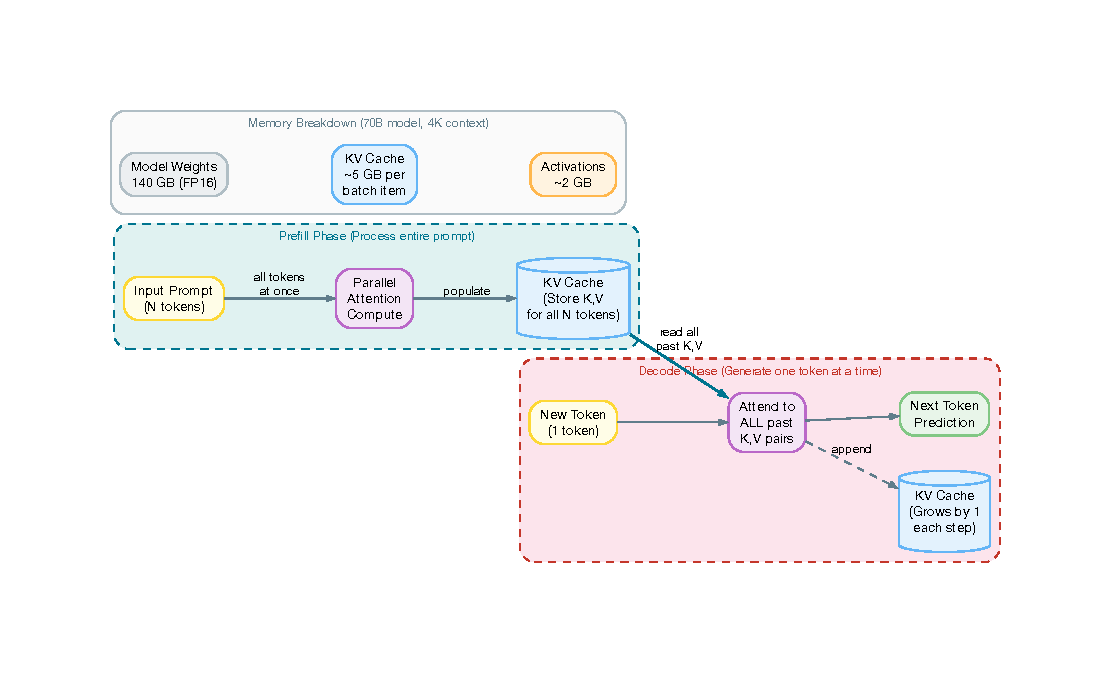
\includegraphics[width=\textwidth]{diagrams/compiled/ch02/kv-cache.pdf}
\caption{KV-cache: prefill vs. decode phases and memory breakdown for inference}
\label{fig:kv-cache}
\end{figure}

The engineering consequence: for a 70B parameter model serving a 4K context window, the KV-cache alone consumes approximately 5GB of GPU memory \emph{per concurrent request}. This means an H100 with 80GB of memory can serve roughly 8 concurrent requests (after accounting for model weights and activations), regardless of the model's theoretical throughput. KV-cache memory, not compute, is typically the bottleneck for LLM serving.

\section{Notable Pre-Training Runs}
\label{sec:notable-runs}


Understanding the design decisions behind major pre-training efforts provides valuable context for engineers working with these models.

\subsection{GPT-4 and the Mixture of Experts Architecture}

GPT-4~\cite{openai2023gpt4} is widely reported to use a Mixture of Experts (MoE) architecture with approximately 1.7 trillion total parameters, but only $\sim$220B parameters are active for any given token (8 experts, 2 active per token). This architecture provides the capacity of a very large model while keeping inference cost closer to that of a $\sim$220B dense model.

From an engineering perspective, MoE introduces additional complexity:
\begin{itemize}[leftmargin=*]
    \item \textbf{Load balancing}: Ensuring tokens are evenly distributed across experts. Imbalanced routing wastes compute and memory on underutilized experts.
    \item \textbf{Expert parallelism}: A new parallelism dimension---different experts on different GPUs---adding to the already complex parallelism strategy.
    \item \textbf{Memory}: All expert weights must be stored, even though only a subset is used per token. This increases memory requirements compared to a dense model of the same active parameter count.
\end{itemize}

\subsection{Gemini: Multimodal Pre-Training}

Google's Gemini~\cite{geminiteam2024gemini} was pre-trained on a mixture of text, images, audio, and video from the start, rather than being adapted from a text-only model. Key engineering decisions:

\begin{itemize}[leftmargin=*]
    \item \textbf{Training infrastructure}: Trained on Google's TPU v4 and v5p pods, using a custom ML framework (JAX/Pax) rather than PyTorch.
    \item \textbf{Multi-modal tokenization}: Different modalities are converted to token sequences using separate encoders (Vision Transformer for images, SoundStream for audio), then interleaved with text tokens.
    \item \textbf{Context length}: 32K tokens at launch, later extended to 1M+ through continued pre-training with longer contexts.
\end{itemize}

\subsection{LLaMA: The Open-Source Catalyst}

Meta's LLaMA~\cite{touvron2023llama} family demonstrated that open-weight models, trained with careful data curation, could match proprietary models at similar parameter counts. Key engineering contributions:

\begin{itemize}[leftmargin=*]
    \item \textbf{RMSNorm}: Using Root Mean Square normalization instead of LayerNorm for better training stability
    \item \textbf{SwiGLU activation}: A more compute-efficient activation function than ReLU
    \item \textbf{RoPE}: Rotary Position Embeddings for better length generalization
    \item \textbf{Grouped Query Attention (GQA)}: Sharing key and value heads across multiple query heads to reduce KV-cache memory at inference time
\end{itemize}

These architectural choices have become the de facto standard for subsequent open-source models (Mistral, Phi, Qwen, etc.).

\section{Chapter Summary}

Pre-training is the foundation of every LLM's capabilities. Understanding this process gives software engineers critical insight into:

\begin{enumerate}[leftmargin=*]
    \item \textbf{Why models behave the way they do}: Their training data determines their knowledge, biases, and blind spots
    \item \textbf{Why tokenization matters}: It directly affects cost, latency, and multilingual performance
    \item \textbf{Why scaling works}: The empirical scaling laws explain why larger models are better and predict future capabilities
    \item \textbf{Why training is expensive}: The infrastructure requirements are staggering, and this cost shapes the entire AI industry
    \item \textbf{Why open-source matters}: Models like LLaMA have democratized access to frontier capabilities
\end{enumerate}

In the next chapter, we turn to what happens \emph{after} pre-training: how raw language models are aligned with human intent through supervised fine-tuning, reinforcement learning from human feedback, and other post-training techniques.
